%% ----------------------------------------------------------------
%% Analysis.tex
%% ---------------------------------------------------------------- 

\chapter{System Analysis} \label{Chapter:System Analysis}

This chapter will focus on the system analysis. Firstly, it will identify the stakeholders of this system. Then, it will introduce a survey used for identifying significant factors influencing the higher education destination choices in the UK and analyse the survey result to identify user requirements. Eventually, this chapter will present the functional requirements and non-functional requirements of this system.


\section{Stakeholders Identification
}

Sommerville \cite{5_sommerville_2011} defined stakeholders are people or organizations who will be affected by the system and who have a direct or indirect influence on the system requirements. Hence, it is necessary to identify stakeholders that are associated with this system. 

The stakeholders of this system will be international students who want to decide destination universities or cities for their higher education in the UK or other people who want to obtain relevant information on higher education in the UK. They can use this system to search for and view information on different cities and universities to help their decision-making process for higher education in the UK.

\section{Survey Design and Analysis
}
In this project, a survey was developed to identify key factors in international students’ decision-making process and analyse the system requirements. This section will firstly introduce the design of the survey and then analyse the results of the survey.


\subsection{Survey Design
}

The survey design was based on the analysis in the section 2.1.1. The respondents of the survey were international students who planned to study in the UK for their higher education. In order to carry out this survey, an online questionnaire hosted in iSurvey was used and distributed to the respondents via emails. The online questionnaire consists of two sections and fifteen questions in total. Section 1 would ask respondents some questions about their educational background, while section 2 used a Likert scale, ranging from no influence to strong influence, to gather their opinions on factors influencing their destination choices for higher education. The online questionnaire can be found in Appendix A.


\subsection{Results Analysis
}

\textbf{Part 1: Profiles of Respondents}

This part will discuss the profiles of 107 respondents in this survey. Figure 4.1 and Figure 4.2 show 64.7\% of respondents continued to pursue their master’s degree in the UK after graduating from universities in their home countries. Besides, 5.6\% of respondents obtained their college diplomas, and 3.7\% of respondents obtained their first master’ degrees before studying in the UK. On the other hand, 25.2\% of respondents choose to study in the UK for their bachelors’ degrees after graduating from high schools.

\begin{figure}[H]
  \centering
  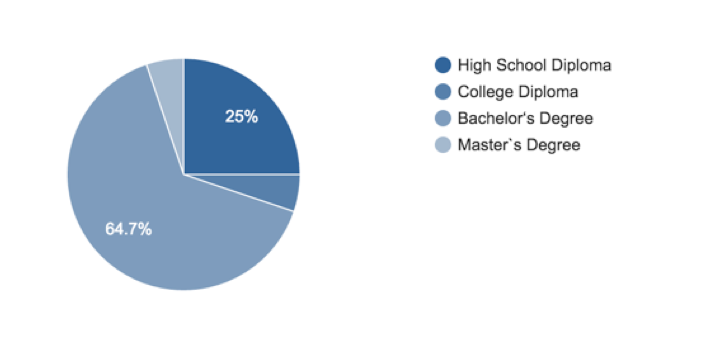
\includegraphics[width=12cm]{./img/Picture4}
  \caption{Highest Level of Education Qualification}
  \label{Figure:figex}
\end{figure}

\begin{figure}[H]
  \centering
  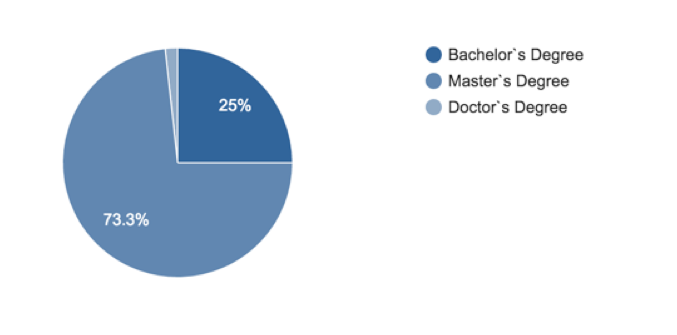
\includegraphics[width=12cm]{./img/Picture5}
  \caption{Level of Education Qualification Pursuing in the UK}
  \label{Figure:figex}
\end{figure}

Figure 4.3 shows most (83.2\%) of respondents choose to study in universities in England (except Greater London), while respondents who choose to study in Greater London, Wales and Scotland only accounted for 6.5\%, 5.6\% and 4.7\% respectively. The main reason was that England (except Greater London) had more universities and lower living expenses compared with Greater London and closer distance to London compared with Wales and Scotland. 

\begin{figure}[H]
  \centering
  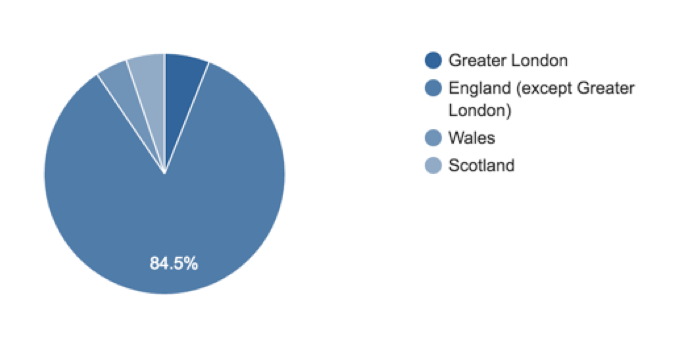
\includegraphics[width=11cm]{./img/Picture6}
  \caption{The Location of University}
  \label{Figure:figex}
\end{figure}

\textbf{Part 2: Perception of the Respondents}

This part will focus on the perception of respondents on different factors in their higher education destination choices. The discussion and analysis in this part will provide a great understanding of factors influencing international student’s higher education destination choices in the UK.

Table 4.1 provides the overview of the perception of respondents regarding what factors have impacts on their destination choices in the UK. It is evident that cost and environment strongly influenced the respondents’ destination higher education choices, and university ranking was considered as a very influential factor in their destination-making process. By contrast, recommendations, employment rate and entry requirements had moderate influences on the respondents’ destination choices, and the least influential factor was international student population. 

\begin{table}[H]
\centering
\caption{Factors Influencing Destination Choices in the UK
}
\label{my-label}
\begin{tabular}{|p{4cm}|c|c|c|c|c|p{2cm}|p{3cm}|}
\hline
                                                                          & \textbf{1} & \textbf{2} & \textbf{3} & \textbf{4} & \textbf{5} & \textbf{Weighted Mean} & \textbf{Interpretation} \\ \hline
University Ranking                                                        & 0          & 1          & 24         & 46         & 36         & 4.09                   & Very Influential        \\ \hline
Cost (tuition fee, living cost, travel cost, etc.)                        & 2          & 0          & 8          & 26         & 71         & 4.53                   & Strongly Influential    \\ \hline
Environment (climate, city size, city location, crime rate of city, etc.) & 2          & 2          & 5          & 20         & 78         & 4.58                   & Strongly Influential    \\ \hline
Recommendations (Word of mouth)                                           & 1          & 22         & 53         & 26         & 5          & 3.11                   & Somewhat Influential    \\ \hline
Entry requirements                                                        & 1          & 17         & 47         & 38         & 4          & 3.24                   & Somewhat Influential    \\ \hline
Employment rate                                                           & 2          & 15         & 44         & 29         & 17         & 3.41                   & Somewhat Influential    \\ \hline
International Student Population                                          & 28         & 51         & 22         & 4          & 2          & 2.07                   & Slightly Influential    \\ \hline
\end{tabular}
\end{table}

In order to get more details about these key factors, some specific questions were included in the online questionnaire. Table 4.2 presents the perception of respondents about university rankings. Because of the reputations and impacts, Times Higher Education university ranking and QS university ranking were considered to be more influential on respondents’ higher education destination choices, even if all rankings about universities in the UK were regarded as very influential factors concerning university rankings.


\begin{table}[H]
\centering
\caption{Influence of Different University Rankings
}
\label{my-label}
\begin{tabular}{|p{4cm}|c|c|c|c|c|p{2cm}|p{3cm}|}
\hline
                                                                   & \textbf{1} & \textbf{2} & \textbf{3} & \textbf{4} & \textbf{5} & \textbf{Weighted Mean} & \textbf{Interpretation} \\ \hline
Guardian University Ranking                                        & 3          & 1          & 25         & 47         & 31         & 3.95                   & Very Influential        \\ \hline
Times Higher Education University Ranking                          & 0          & 4          & 11         & 30         & 62         & 4.4                    & Very Influential        \\ \hline
QS University Ranking                                              & 0          & 1          & 14         & 31         & 61         & 4.45                   & Very Influential        \\ \hline
US News Global Universities Ranking                                & 2          & 46         & 35         & 20         & 4          & 2.79                   & Somewhat Influential    \\ \hline
Research Excellence Framework (REF)                                & 1          & 3          & 16         & 52         & 35         & 4.09                   & Very Influential        \\ \hline
The Complete University Guide Ranking (CUG)                        & 2          & 4          & 45         & 45         & 11         & 3.55                   & Very Influential        \\ \hline
Academic Ranking of World Universities (Shanghai JiaoTong Ranking) & 67         & 24         & 9          & 4          & 3          & 1.62                   & Slightly Influential    \\ \hline
\end{tabular}
\end{table}

Table 4.3 illustrates the perception of respondents regarding different expenses, such as tuition fees, living costs and travel costs. It was evident that travel expenses had fewer impacts on the respondents’ decision-making process for higher education, compared with tuition fees and living costs. 

\begin{table}[H]
\centering
\caption{Influence of Different Expenses}
\label{my-label}
\begin{tabular}{|p{4cm}|c|c|c|c|c|p{2cm}|p{3cm}|}
\hline
            & \textbf{1} & \textbf{2} & \textbf{3} & \textbf{4} & \textbf{5} & \textbf{Weighted Mean} & \textbf{Interpretation} \\ \hline
Tuition fee & 1          & 1          & 3          & 31         & 71         & 4.58                   & Strongly Influential    \\ \hline
Living cost & 1          & 1          & 8          & 29         & 68         & 4.51                   & Strongly Influential    \\ \hline
Travel cost & 3          & 27         & 51         & 23         & 3          & 2.96                   & Somewhat Influential    \\ \hline
\end{tabular}
\end{table}

Table 4.4 shows the perception of the respondents on different environmental factors. Information on the safety and location of the city were regarded as two strongly influential factors in the respondents’ decision-making process. Moreover, other information on cities, such as size, location and infrastructure were also considered in their decision making.


\begin{table}[H]
\centering
\caption{Influence of Different Environmental Factors
}
\label{my-label}
\begin{tabular}{|p{4cm}|c|c|c|c|c|p{2cm}|p{3cm}|}
\hline
                                                               & \textbf{1} & \textbf{2} & \textbf{3} & \textbf{4} & \textbf{5} & \textbf{Weighted Mean} & \textbf{Interpretation} \\ \hline
Campus environment                                             & 1          & 2          & 54         & 41         & 9          & 3.5                    & Very Influential        \\ \hline
Climate (weather)                                              & 2          & 3          & 9          & 50         & 43         & 4.2                    & Very Influential        \\ \hline
Safety of the city                                             & 1          & 1          & 9          & 33         & 63         & 4.46                   & Strongly Influential    \\ \hline
City size                                                      & 3          & 0          & 36         & 23         & 45         & 4                      & Very Influential        \\ \hline
City location (geographic proximity to capital city or London) & 0          & 1          & 14         & 19         & 73         & 4.53                   & Strongly Influential    \\ \hline
City infrastructure (airport, railway station, etc.)           & 2          & 8          & 21         & 20         & 56         & 4.12                   & Very Influential        \\ \hline
\end{tabular}
\end{table}


Table 4.5 provides the perception of the respondents on recommendations or word-of-mouth. It can be seen that recommendations from agents and official website were more influential than those from the respondents’ parents and friends.

\begin{table}[H]
\centering
\caption{Influence of Recommendations From Different People
}
\label{my-label}
\begin{tabular}{|p{4cm}|c|c|c|c|c|p{2cm}|p{3cm}|}
\hline
                            & \textbf{1} & \textbf{2} & \textbf{3} & \textbf{4} & \textbf{5} & \textbf{Weighted Mean} & \textbf{Interpretation} \\ \hline
Parents/Relatives           & 2          & 5          & 17         & 55         & 28         & 3.95                   & Very Influential        \\ \hline
Friends                     & 2          & 4          & 18         & 65         & 18         & 3.87                   & Very Influential        \\ \hline
Agents                      & 3          & 7          & 13         & 31         & 53         & 4.15                   & Very Influential        \\ \hline
University official website & 2          & 4          & 9          & 29         & 63         & 4.37                   & Very Influential        \\ \hline
\end{tabular}
\end{table}


To summarize, the key factors in the international students’ decision-making process for higher education are “university ranking”, “cost” and “environment”. Therefore, information on these three factors should be contained in the system. Specifically, there is no great difference between universities rankings when the international students want to know the reputation of universities as long as these rankings are about universities in the UK. In term of costs, the international students pay much more attention to tuition fees and living expenses, so information on these two types of costs should be provided in this system. Besides, the information on safety and location of cities should also be included in the system to provide information on the environment for international students’ higher education destination choices in the UK. 

\section{User Requirements
}

Based on the analysis above, we can identify user requirements that the stakeholders expect in this system in Table 4.6.

\begin{table}[H]
\centering
\caption{User Requirements of This System
}
\label{my-label}
\begin{tabular}{|p{2cm}|p{11cm}|}
\hline
\textbf{Identifier} & \textbf{User Requirement}                                                                                                               \\ \hline
UREQ1               & As an international student, I want to search for the universities and programs in the UK.                                              \\ \hline
UREQ2               & As an international student, I want to know the ranking of a certain university.                                                        \\ \hline
UREQ3               & As an international student, I want to know the tuition fee in a certain university or city.                                            \\ \hline
UREQ4               & As an international student, I want to know the living expense in the city that a certain university is located in                      \\ \hline
UREQ5               & As an international student, I want to know the employment rate of a certain program                                                    \\ \hline
UREQ6               & As an international student, I want to know the entry requirement of a certain program                                                  \\ \hline
UREQ7               & As an international student, I want to know the campus environment of a certain university.                                             \\ \hline
UREQ8               & As an international student, I want to know the location of a certain university.                                                       \\ \hline
UREQ9               & As an international student, I want to know the geographic proximity of this university to capital city or London.                      \\ \hline
UREQ10              & As an international student, I want to know the size of the city that a certain university is located in.                               \\ \hline
UREQ11              & As an international student, I want to know the climate or weather of the city that a certain university is located in.                 \\ \hline
UREQ12              & As an international student, I want to know the information on criminality in the city that a certain university is located in.         \\ \hline
UREQ13              & As an international student, I want to know the infrastructure in the city that a certain university is located in.                     \\ \hline
UREQ14              & As an international student, I want to share information on a certain university or program to get some advice from parents or friends. \\ \hline
UREQ15              & As an international student, I want to know some information on a certain university or program from its official website.              \\ \hline
\end{tabular}
\end{table}


\section{System Requirements
}

\subsection{Functional Requirements
}

The functional requirements of this system are derived from the above user requirements. Table 4.7 displays the functional requirements with their descriptions. Due to time constraints, the requirements are categorized into high, medium and low. The implementation will focus the requirements with high priority to achieve the system’s main objectives.

\begin{table}[H]
\centering
\caption{Functional Requirements of This System
}
\label{my-label}
\begin{tabular}{|p{2cm}|p{3cm}|p{1.5cm}|p{7cm}|}
\hline
\textbf{Identifier} & \textbf{Related User Requirement}         & \textbf{Priority} & \textbf{Description}                                                                                                              \\ \hline
FRQ1                & UREQ1, UREQ3, UREQ4, UREQ5, UREQ6, UREQ15 & High              & The system shall allow users to search for universities or programs and offer users relevant information on them.                 \\ \hline
FRQ2                & UREQ2                                     & High              & The system shall allow users to know the ranking of a certain university.                                                         \\ \hline
FRQ3                & UREQ7, UREQ8, UREQ9                       & High              & The system shall allow users to know the campus environment, the location and the geographic proximity of a certain university    \\ \hline
FRQ4                & UREQ10                                    & Medium            & The system shall allow users to know the size of the city that a certain university is located in                                 \\ \hline
FRQ5                & UREQ11                                    & High              & The system shall allow users to know the climate or weather of the city that a certain university is located in.                  \\ \hline
FRQ6                & UREQ12                                    & High              & The system shall allow users to know the information  on criminality in the city that a certain university is located in is safe. \\ \hline
FRQ7                & UREQ13                                    & High              & The system shall allow users to know the infrastructure in the city that a certain university is located in.                      \\ \hline
FRQ8                & UREQ14                                    & Medium            & The system shall allow users to share information on a certain university or program to get some advice from parents or friends.  \\ \hline
\end{tabular}
\end{table}


\subsection{Non-functional Requirements
}

Apart from functional requirements, the non-functional requirements should be taken into consideration during the design and implementation stages. Table 4.8 displays the non-functional requirements that should be complied with to build a high-quality system.

\begin{table}[H]
\centering
\caption{Non-functional Requirements of This System}
\label{my-label}
\begin{tabular}{|p{2cm}|p{3cm}|p{8cm}|}
\hline
\textbf{Identifier} & \textbf{Type}   & \textbf{Description}                                                                                                             \\ \hline
NRQ1                & Usability       & The interface of this system should be well structured or easy to learn and understand.                                          \\ \hline
NRQ2                & Usability       & The interface of this system should be responsive or be able to adjust itself on different devices (PC, smartphones and tablets) \\ \hline
NRQ3                & Accessibility   & The design of this system should comply with Web accessibility standards provided by W3C.                                        \\ \hline
NRQ4                & Availability    & The system should be available  95\% of the time for any day.                                                                    \\ \hline
NRQ5                & Compatibility   & The system should be compatible with commonly-used web browsers (Chrome, Firefox, IE and Safari)                                    \\ \hline
NRQ6                & Maintainability & The code of this system should be easy to maintain. The usage of MVVM pattern can ensure this system is easy to maintain.                                                                              \\ \hline
%NRQ7                & Performance     & The system should be able to handle ten requests per second.                                                                     \\ \hline
\end{tabular}
\end{table}


\section{Summary}
This chapter provides information on the system analysis. It consists of the stakeholders of this system, the user requirements, the system requirements (functional and non-functional requirements). Besides, the survey designed for identifying key factors in international students’ decision-making process is introduced and analysed to determine the user requirements of this system.


